\documentclass[10pt]{article}

\usepackage[margin=0.75in]{geometry}
\usepackage[T1]{fontenc}
\usepackage{lmodern}
\usepackage{microtype}
\usepackage{graphicx}
\usepackage{enumitem}
\usepackage[dvipsnames]{xcolor}
\usepackage{titlesec}
\definecolor{linkblue}{HTML}{1A5FB4}
\definecolor{ink}{HTML}{1F3A5F}
\usepackage[colorlinks=true,urlcolor=linkblue,linkcolor=linkblue]{hyperref}

\pagestyle{empty}
\setlength{\parindent}{0pt}
\setlength{\parskip}{0.35em}
\setlist{itemsep=0.1em,topsep=0.2em,leftmargin=1.2em}
\titleformat{\section}{\normalfont\normalsize\bfseries\color{ink}}{}{0em}{}
\titlespacing*{\section}{0pt}{0.7em}{0.2em}

\begin{document}

{\LARGE\bfseries\color{ink} State Shock Ledger}\hfill{\small Prototype version 0, October 2026}\\[0.3em]
{\large How world commodity prices move income between U.S.\ states}\\[0.2em]
\rule{\textwidth}{0.6pt}

When the world price of oil, natural gas, grain or cattle changes, income moves between
American states, because some states produce far more of a commodity than they use and
others use far more than they produce. The State Shock Ledger measures each state's gain
or loss, in dollars and as a share of the state's economy, for all fifty states and the
District of Columbia, using one consistent method and only public data.

\section{What it shows}
\begin{itemize}
  \item \textbf{Latest:} each state's windfall from the past year's price change; energy
  updated daily from EIA spot prices.
  \item \textbf{History:} monthly since January 2000, so any price episode can be compared
  with earlier ones (2008, 2014 to 2016, 2020, 2022).
  \item \textbf{Outlook:} the energy windfall implied by EIA's Short-Term Energy Outlook.
  \item \textbf{Scenario:} set oil and gas prices and see every state's exposure.
  \item \textbf{The ledger:} which states gain and which pay, side by side.
\end{itemize}

\begin{center}
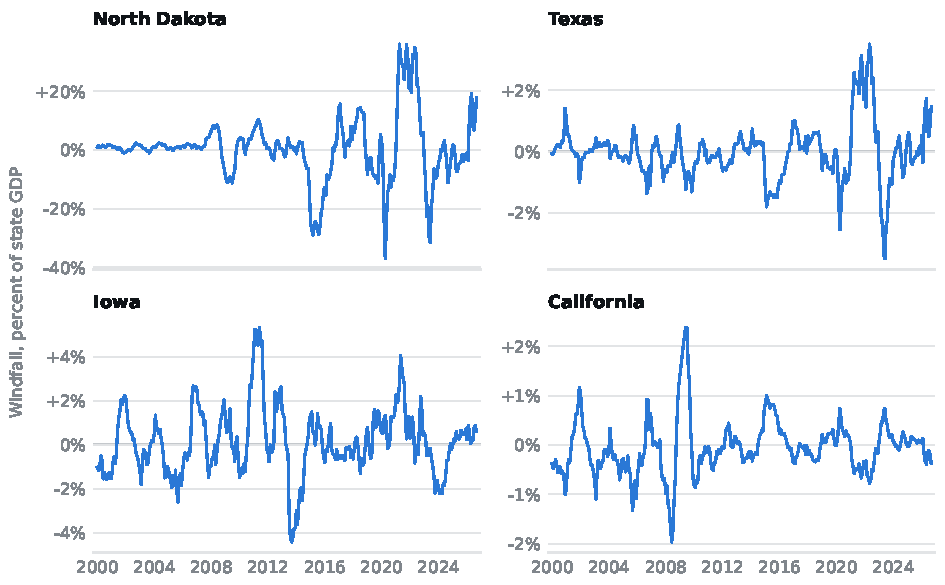
\includegraphics[width=0.92\textwidth,height=2.35in,keepaspectratio]{fig_states.pdf}\\[-0.2em]
{\footnotesize Monthly windfall, percent of state GDP, 2000 to 2026. Scales differ across panels.}
\end{center}

\section{Who it is for}
State budget and legislative fiscal offices (revenue exposure and forecasting); federal
analysts weighing energy assistance, Strategic Petroleum Reserve releases or farm support
(where the burden of a price shock falls); researchers (an open state-level dataset).

\section{How it works}
For each state and commodity, the net position (production minus consumption, averaged
over the three prior years) is multiplied by the change in the world price. Crude oil and
natural gas cover both producers and consumers; corn, soybeans, wheat and cattle cover
producers in this version. Sources: EIA State Energy Data System and daily prices, USDA
Economic Research Service farm receipts, World Bank commodity prices, BEA state GDP.
Figures are gross values at benchmark prices, an upper bound on income in the state.
A methods note documents every definition and limitation.

\section{Status and next steps}
Working prototype. Next: copper, potash and coal; the consumer side of food prices; and
estimates of what each state's windfall implies for its jobs, income and tax revenue.
Feedback on what would make it useful to your work is very welcome.

\vfill
\rule{\textwidth}{0.4pt}\\
{\small Samson M'boueke, Ph.D.\ in Economics, University of Notre Dame\\
Dashboard: \fbox{\strut public address to be added} \qquad Contact: \fbox{\strut email}}

\end{document}
